\section{歪曲収差以外の収差とその特徴について}
1章にて、収差には単色収差と色収差が存在すると述べた。また、単色収差にはザイデルの5収差がある。
\subsection{ザイデルの5収差}
\subsubsection{球面収差}
球面収差とは、レンズ面が球面であることにより発生する収差である。
%球面収差とは、光軸から離れた光線ほど、光学系浸透後に、軸上での像点が手前にできてしまうことをいう。他の収差と異なり、像面全体に同量の収差を生じさせる。また光軸上の物体に対しても収差が存在するのは、球面収差だけとなってである。
\begin{figure}[h]
	\centering
	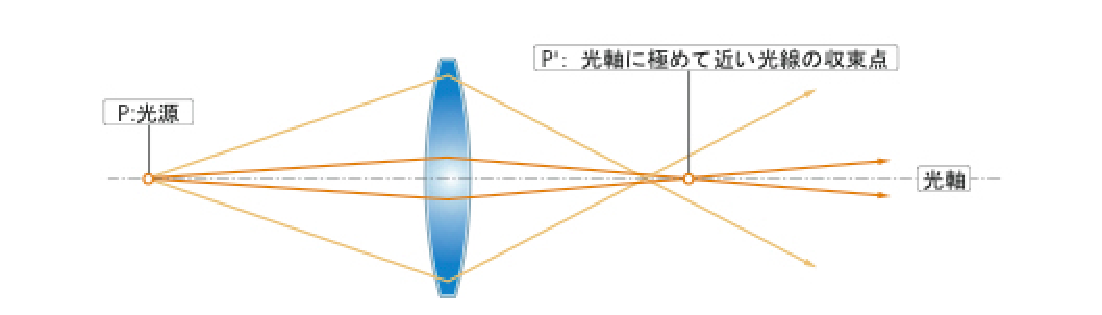
\includegraphics[height=30mm]{image/kyumen.png.eps}
	\caption{球面収差\ \cite{cite1}}
	\label{caption1}
\end{figure}

\subsubsection{コマ収差}
コマ収差とは、光軸より離れた物点の横倍率が物点の位置により異なる収差のことをいう。
\begin{figure}[h]
	\centering
	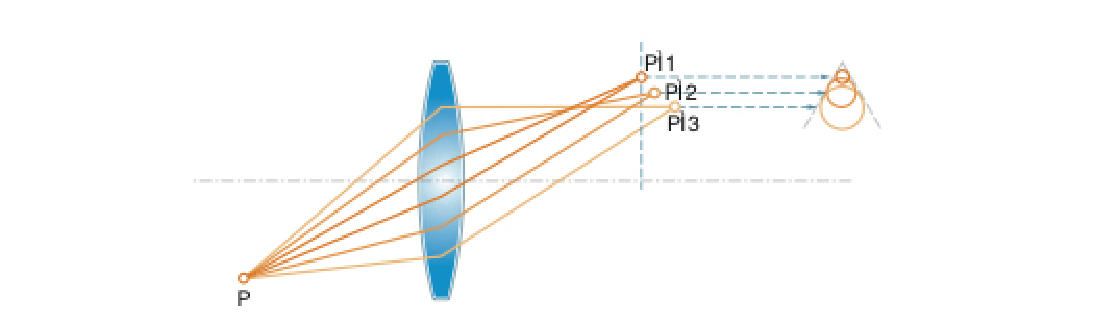
\includegraphics[height=30mm]{image/koma.png.eps}
	\caption{コマ収差\ \cite{cite1}}
	\label{caption1}
\end{figure}

\subsubsection{非点収差}
非点収差とは、子午光線と球欠光線に対する焦点距離の違いのことをいう。
\begin{figure}[h]
	\centering
	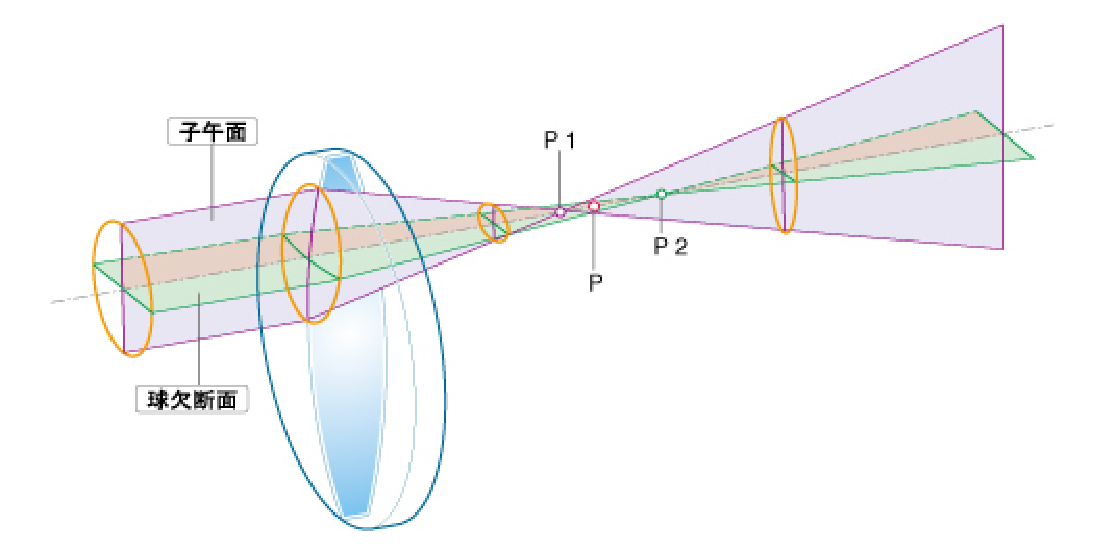
\includegraphics[height=40mm]{image/hiten.png.eps}
	\caption{非点収差}
	\label{caption1}
\end{figure}


\subsubsection{像面収差}
像面収差とは、光軸に平行な光線と傾いた光線が、光軸に垂直な同一面に結像しないことをいう。
\begin{figure}[h]
	\centering
	
\includegraphics[width=50mm]{image/dummy.png.eps}
	\caption{像面収差}
	\label{caption1}
\end{figure}

\subsection{色収差}